%\PassOptionsToClass{handout}{beamer}
\documentclass[aspectratio=169,usepdftitle=true]{beamer}
\usefonttheme{professionalfonts}

\usepackage[T1]{fontenc}
\usepackage[utf8]{luainputenc}
%\usepackage[utf8]{inputenc}
\usepackage{microtype}
\usepackage{unicode-math}
\setmathfont{latinmodern-math.otf}
\usepackage{csquotes}
\usepackage[ngerman]{babel}
\usepackage{lipsum}
\usepackage{listings}
\usepackage[backend=biber,style=alphabetic]{biblatex}
\addbibresource{example.bib}

\usetheme{dividing-lines}
\SetColorProfile{159, 166, 2}{249, 224, 176}{137, 164, 75}

\title{Neuronale Netze}
\subtitle{Handschriftliche Zahlen erkennen}
\institute{Carl-Friedrich-Gauß-Gymnasium}
\license{\ccbysa}

\date{\today}

\author{Jasper Gude}
%\email{j.gude@posteo.de}
\outro{Hockenheim, \today}
\license[]{\url{https://creativecommons.org/licenses/by-sa/4.0/}\quad\ccbysa}

% just an example command
\newcommand\twosplit[3][c]{%
\begin{columns}[#1]
\begin{column}{0.475\linewidth}#2\end{column}\hfill
\begin{column}{0.475\linewidth}#3\end{column}
\end{columns}}


\def\mnistAnimated#1{
\resizebox{\linewidth}{!}{
\begin{tikzpicture}
\node[inner sep=0pt] (pic) at (28px,28px) {\includegraphics[width = 56px]{#1}};
\draw[lightgray,thin] (0,0) rectangle (56px,56px);
\onslide<2->{\draw[step=2px,lightgray,ultra thin] (0,0) grid (56px,56px);}
\end{tikzpicture}}
}

\def\mnist#1{
\resizebox{\linewidth}{!}{
\begin{tikzpicture}
\node[inner sep=0pt] (pic) at (28px,28px) {\includegraphics[width = 56px]{#1}};
\draw[lightgray,thin] (0,0) rectangle (56px,56px);
\draw[step=2px,lightgray,ultra thin] (0,0) grid (56px,56px);
\end{tikzpicture}}
}

\def\neuralnetworkAnimated{
\begin{tikzpicture}[bc/.default={lgray}]
\onslide<3->{
\foreach \i in {0,...,9}
    \node[bc, text width = 0.1, fill = none, draw=btdl@color@black, label = {right:\i}] (o\i) at (12,0.5*\i+1.75) {};
}
\onslide<4->{
\foreach \i in {0,...,15}{
    \node[bc, text width = 0.1, fill = none, draw=btdl@color@black] (h\i) at (8,0.5*\i+0.25) {};
    \onslide<5->{
    \foreach \j in {0,...,9}
        \draw[ultra thin] (h\i) -- (o\j);}
}
\foreach \i in {0,...,15}{
    \node[bc, text width = 0.1, fill = none, draw=btdl@color@black] (i\i) at (4,0.5*\i+0.25) {};
    \onslide<5->{
    \foreach \j in {0,...,15}
        \draw[ultra thin] (i\i) -- (h\j);}
}
}
\onslide<2->{
\foreach \i in {0,...,7}{
    \node[bc, text width = 0.1, fill = none, draw=btdl@color@black] (x\i) at (0,0.5*\i) {};
        \onslide<5->{
        \foreach \j in {0,...,15}
        \draw[ultra thin] (x\i) -- (i\j);}
}
\node[ fill = none, draw=none] (x8) at (0,0.5*8) {$\vdots$};
\foreach \i in {9,...,16}{
    \node[bc, text width = 0.1, fill = none, draw=btdl@color@black] (x\i) at (0,0.5*\i) {};
    \onslide<5->{
    \foreach \j in {0,...,15}
        \draw[ultra thin] (x\i) -- (i\j);}
}
\draw[decoration={brace,raise=20pt},decorate] (x0) -- node[left=20pt] {784} (x16);
}
\end{tikzpicture}
}

\def\neuralnetworkSingleNeuron{
\begin{tikzpicture}[bc/.default={lgray}]
    \node[bc, text width = 0.1, fill = none, draw=btdl@color@black] (i0) at (4,-0.5*8) {};

\foreach \i in {0,...,7}{
    \node[bc, text width = 0.1, fill = none, draw=btdl@color@black, label = {right:$x_\i$}] (x\i) at (0,-0.5*\i) {};
    \draw[ultra thin] (x\i) -- (i0);
    \node (w\i) at (2,-0.5*\i) {$w_\i$};
}
\node[fill = none, draw=none, label = {right:$x_n$}] (x8) at (0,-0.5*8) {$\vdots$};
\node (wn) at (2,-0.5*8) {$w_n$};
\foreach \i in {9,...,16}{
    \node[bc, text width = 0.1, fill = none, draw=btdl@color@black] (x\i) at (0,-0.5*\i) {};
    \draw[ultra thin] (x\i) -- (i0);
}
\draw[decoration={brace,raise=20pt},decorate] (x16) -- node[left=20pt] {784} (x0);
\end{tikzpicture}
}

\def\perceptron{
\begin{tikzpicture}[bc/.default={lgray}]
    \node[] (x0) at (-4,2) {$x_0$};
    \node[] (x1) at (-4,1) {$x_1$};
    \node[] (x2) at (-4,0) {$x_2$};
    \node[] (x...) at (-4,-1) {...};
    \node[] (xn) at (-4,-2) {$x_n$};
    \node[above=.75cm, text width=8em, align=center] at (x0) {Inputvektor $\vec{x}$};

    \node[bc, rectangle, minimum size=1cm] (ueber) at (0,0) {$\sum$};
    \node[below=.75cm, text width=8em, align=center] at (ueber) {Übertragungsfunktion};


    \draw[ctarrow=lgray] (x0) -- (ueber) node[text=darkgray,midway] {$ w_{0 }$};
    \draw[ctarrow=lgray] (x1) -- (ueber) node[text=darkgray,midway] {$ w_{1 }$};
    \draw[ctarrow=lgray] (x2) -- (ueber) node[text=darkgray,midway] {$ w_{2 }$};
    \draw[ctarrow=lgray] (xn) -- (ueber) node[text=darkgray,midway] {$ w_{n }$};

    \node[bc, rectangle, minimum size=1cm] (aktiv) at (4,0) {$\varphi$};
    \node[below=.75cm, text width=8em, align=center] at (aktiv) {Aktivierungsfunktion};

    \draw[tarrow=lgray] (ueber) -- (aktiv) node[text=darkgray,midway] (net) {$net$};
    \node[above=.75cm, text width=8em, align=center] at (net) {Netzeingabe};

    \node[] (out) at (6,0) {$o$};
    \node[above=.75cm, text width=8em, align=center] at (out) {Output};
    \draw[tarrow=lgray] (aktiv) -- (out);
\end{tikzpicture}}

\def\perceptronFirstHalf{
\begin{tikzpicture}[bc/.default={lgray}]
    \node[] (x0) at (-4,2) {$x_0$};
    \node[] (x1) at (-4,1) {$x_1$};
    \node[] (x2) at (-4,0) {$x_2$};
    \node[] (x...) at (-4,-1) {...};
    \node[] (xn) at (-4,-2) {$x_n$};
    \node[above=.75cm, text width=8em, align=center] at (x0) {Inputvektor $\vec{x}$};

    \node[bc, rectangle, minimum size=1cm] (ueber) at (0,0) {$\sum$};
    \node[below=.75cm, text width=8em, align=center] at (ueber) {Übertragungsfunktion};


    \draw[ctarrow=lgray] (x0) -- (ueber) node[text=darkgray,midway] {$ w_{0 }$};
    \draw[ctarrow=lgray] (x1) -- (ueber) node[text=darkgray,midway] {$ w_{1 }$};
    \draw[ctarrow=lgray] (x2) -- (ueber) node[text=darkgray,midway] {$ w_{2 }$};
    \draw[ctarrow=lgray] (xn) -- (ueber) node[text=darkgray,midway] {$ w_{n }$};


    \draw[tarrow=lgray] (ueber) -- (2,0) node[text=darkgray,midway] (net) {$net$};
    \node[above=.75cm, text width=8em, align=center] at (net) {Netzeingabe};
\end{tikzpicture}}

\def\perceptronSecondHalf{
\begin{tikzpicture}[bc/.default={lgray}]
    \node[bc, rectangle, minimum size=1cm] (aktiv) at (4,0) {$\varphi$};
    \node[below=.75cm, text width=8em, align=center] at (aktiv) {Aktivierungsfunktion};

    \draw[tarrow=lgray] (2,0) -- (aktiv) node[text=darkgray,midway] (net) {$net$};
    \node[above=.75cm, text width=8em, align=center] at (net) {Netzeingabe};

    \node[] (out) at (6,0) {$o$};
    \node[above=.75cm, text width=8em, align=center] at (out) {Output};
    \draw[tarrow=lgray] (aktiv) -- (out);
\end{tikzpicture}}

\def\feedforwardNetwork{
\begin{tikzpicture}[bc/.default={lgray}]
    \node[bc] (x0) at (-4,1) {$x_0$};
    \node[bc] (x1) at (-4,0) {$x_1$};
    \node[bc] (x2) at (-4,-1) {$x_2$};

    \node[bc, fill=btdl@color@secondary] (neuro0) at (0,1) {};
    \node[bc, fill=btdl@color@secondary] (neuro1) at (0,0) {};
    \node[bc, fill=btdl@color@secondary] (neuro2) at (0,-1) {};
    \node[below=.75cm, text width=8em, align=center] at (neuro2) {Ausgabeschicht};

    \draw[tarrow=lgray] (x0) -- (neuro0);
    \draw[tarrow=lgray] (x0) -- (neuro1);
    \draw[tarrow=lgray] (x0) -- (neuro2);

    \draw[tarrow=lgray] (x1) -- (neuro0);
    \draw[tarrow=lgray] (x1) -- (neuro1);
    \draw[tarrow=lgray] (x1) -- (neuro2);

    \draw[tarrow=lgray] (x2) -- (neuro0);
    \draw[tarrow=lgray] (x2) -- (neuro1);
    \draw[tarrow=lgray] (x2) -- (neuro2);

    \node[] (o0) at (2,1) {};
    \node[] (o1) at (2,0) {};
    \node[] (o2) at (2,-1) {};

    \draw[tarrow=lgray] (neuro0) -- (o0);
    \draw[tarrow=lgray] (neuro1) -- (o1);
    \draw[tarrow=lgray] (neuro2) -- (o2);

\end{tikzpicture}}

\def\deepfeedforwardNetwork{
\begin{tikzpicture}[bc/.default={lgray}]
    \node[bc] (x0) at (-4,1) {$x_0$};
    \node[bc] (x1) at (-4,0) {$x_1$};
    \node[bc] (x2) at (-4,-1) {$x_2$};

    \node[bc, fill=btdl@color@primary] (neuro00) at (0,1) {};
    \node[bc, fill=btdl@color@primary] (neuro10) at (0,0) {};
    \node[bc, fill=btdl@color@primary] (neuro20) at (0,-1) {};
    \node[below=.75cm, text width=10em, align=center] at (neuro20) {verborgene Schicht};

    \draw[tarrow=lgray] (x0) -- (neuro00);
    \draw[tarrow=lgray] (x0) -- (neuro10);
    \draw[tarrow=lgray] (x0) -- (neuro20);

    \draw[tarrow=lgray] (x1) -- (neuro00);
    \draw[tarrow=lgray] (x1) -- (neuro10);
    \draw[tarrow=lgray] (x1) -- (neuro20);

    \draw[tarrow=lgray] (x2) -- (neuro00);
    \draw[tarrow=lgray] (x2) -- (neuro10);
    \draw[tarrow=lgray] (x2) -- (neuro20);

    \node[bc, fill=btdl@color@secondary] (neuro01) at (4,0.5) {};
    \node[bc, fill=btdl@color@secondary] (neuro11) at (4,-0.5) {};

    \draw[tarrow=lgray] (neuro00) -- (neuro01);
    \draw[tarrow=lgray] (neuro00) -- (neuro11);

    \draw[tarrow=lgray] (neuro10) -- (neuro01);
    \draw[tarrow=lgray] (neuro10) -- (neuro11);

    \draw[tarrow=lgray] (neuro20) -- (neuro01);
    \draw[tarrow=lgray] (neuro20) -- (neuro11);

    \node[] (o0) at (6,0.5) {};
    \node[] (o1) at (6,-0.5) {};
    \node[below=.75cm, text width=8em, align=center] at (neuro11) {Ausgabeschicht};


    \draw[tarrow=lgray] (neuro01) -- (o0);
    \draw[tarrow=lgray] (neuro11) -- (o1);

\end{tikzpicture}}

\def\recursiveNetwork{
\begin{tikzpicture}[bc/.default={lgray}]
    \node[bc] (x0) at (-4,1.5) {$x_0$};
    \node[bc] (x1) at (-4,0.5) {$x_1$};
    \node[bc] (x2) at (-4,-0.5) {$x_2$};
    \node[bc] (x3) at (-4,-1.5) {$x_3$};

    \node[bc, fill=btdl@color@secondary] (neuro00) at (0,1.5) {};
    \node[bc, fill=btdl@color@secondary] (neuro10) at (0,0) {};
    \node[bc, fill=btdl@color@secondary] (neuro20) at (0,-1.5) {};
    \node[below=.75cm, text width=8em, align=center] at (neuro20) {Ausgabeschicht};

    \draw[tarrow=lgray] (x0) -- (neuro00);
    \draw[tarrow=lgray] (x0) -- (neuro10);
    \draw[tarrow=lgray] (x0) -- (neuro20);

    \draw[tarrow=lgray] (x1) -- (neuro00);
    \draw[tarrow=lgray] (x1) -- (neuro10);
    \draw[tarrow=lgray] (x1) -- (neuro20);

    \draw[tarrow=lgray] (x2) -- (neuro00);
    \draw[tarrow=lgray] (x2) -- (neuro10);
    \draw[tarrow=lgray] (x2) -- (neuro20);

    \draw[tarrow=lgray] (x2) -- (neuro00);
    \draw[tarrow=lgray] (x2) -- (neuro10);
    \draw[tarrow=lgray] (x2) -- (neuro20);

    \draw[tarrow=lgray] (x3) -- (neuro00);
    \draw[tarrow=lgray] (x3) -- (neuro10);
    \draw[tarrow=lgray] (x3) -- (neuro20);

    \node[] (o0) at (2,1.5) {};
    \node[] (o1) at (2,0) {};
    \node[] (o2) at (2,-1.5) {};

    \draw[tarrow=lgray] (neuro00) -- (o0);
    \draw[tarrow=lgray] (neuro00.east) .. controls +(right:1) and +(up:1) .. (neuro00.north);

    \draw[tarrow=lgray] (neuro10) -- (o1);
    \draw[tarrow=lgray] (neuro10.east) .. controls +(right:1) and +(up:1) .. (neuro10.north);

    \draw[tarrow=lgray] (neuro20) -- (o2);
    \draw[tarrow=lgray] (neuro20.east) .. controls +(right:1) and +(up:1) .. (neuro20.north);

\end{tikzpicture}}


\def\typesetBox#1#2#3#4{%
    \pbox{7cm}{{\Large\sbfamily#1}\rlap{\textsuperscript{\color{gray}\cite{#4}}}\\\color{gray}#2\hfill#3}%
}

\definecolor{btdl@color@red}{RGB}{163, 75, 102}
\colorlet{semigray}{gray!70!darkgray}
\lstset{
    backgroundcolor=\color{btdl@color@black},
    commentstyle=\color{semigray},
    keywordstyle=\bfseries\color{btdl@color@primary},
    numberstyle=\tiny\color{semigray},
    stringstyle=\color{btdl@color@secondary},
    basicstyle=\ttfamily\color{btdl@color@white},
    breakatwhitespace=false,
    breaklines=true,
    captionpos=b,
    keepspaces=true,
    numbers=left,
    numbersep=5pt,
    showspaces=false,
    showstringspaces=false,
    showtabs=false,
    tabsize=2
}

\usetikzlibrary{arrows.meta,calc,backgrounds,shapes.multipart,intersections,positioning,decorations.pathreplacing}
\tikzset{
    bc/.style={circle,draw,fill,#1,text=darkgray,align=center,text width=0.75em},
    brs/.style={rectangle,rounded corners=2.5pt,draw,fill,#1,text=darkgray,align=center},
    br/.style={brs=#1,rectangle split,rectangle split parts=2,draw=btdl@color@background,thick,font=\scriptsize\sffamily},
    br/.default={hl-shade},
    bcsmall/.style={circle,draw,fill,#1,text=darkgray,align=center,inner sep=2pt},
    bc/.default={hl-shade},
    bcsmall/.default={hl-shade},
    t/.style={ultra thick,#1},
    tarrow/.style={-Kite,t=#1},
    dtarrow/.style={Kite-Kite,t=#1},
    ctarrow/.style={Circle-Kite,t=#1}
}


\def\cfl#1{\faFile\llap{\color{#1}\tiny\faCogs\;}}
\def\tagS#1#2{\node[above left=-0.082cm,darkgray,scale=0.65,circle,fill=lgray,inner sep=1pt] at(#1.south east) {\sbfamily#2};}
\def\tagN#1#2{\node[below left=-0.082cm,darkgray,scale=0.65,circle,fill=hl-shade,inner sep=1pt] at(#1.north east) {\sbfamily#2};}

\colorlet{lgray}{lightgray!45!white}
\colorlet{hl-shade}{btdl@color@secondary}

\usepackage{pgfplots}
\pgfplotsset{width=\linewidth}

\begin{document}
\section{Modellierung}
\begin{frame}{Modellierung des Problems}
\begin{layout-imageonly}
\begin{columns}[c]
\begin{column}{0.3\linewidth}
\centering
\mnistAnimated{Mnist3-a.png}
\end{column}\hfill
\begin{column}{0.3\linewidth}
\centering
\mnistAnimated{Mnist3-b.png}
\end{column}\hfill
\begin{column}{0.3\linewidth}
\centering
\mnistAnimated{Mnist3-c.png}
\end{column}
\end{columns}
\centering
\onslide<3->{
\begin{tikzpicture}[bc/.default={lgray}]
\node[rectangle,draw=lgray, fill=white, text=black, align=center, minimum size=1.5cm ] (w) at (0,0) {0,00};
\node[rectangle, fill=white!75!black, text=black, align=center, minimum size=1.5cm,  right=1cm of w] (lg) {0,25};
\node[rectangle, fill=white!50!black, text=white, align=center, minimum size=1.5cm,  right=1cm of lg] (g) {0,50};
\node[rectangle, fill=white!25!black, text=white, align=center, minimum size=1.5cm,  right=1cm of g] (dg) {0,75};
\node[rectangle, fill=black, text=white, align=center, minimum size=1.5cm, right=1cm of dg ] {1,00};
\end{tikzpicture}
}
\end{layout-imageonly}
\end{frame}

\begin{frame}{Überführung auf eine Netzstruktur}
\begin{layout-imageonly}
\begin{columns}[c]
\begin{column}{0.3\linewidth}
\centering
\mnist{Mnist3-a.png}
28px $\times$ 28px
\end{column}\hfill
\begin{column}{0.7\linewidth}
\centering
\resizebox{!}{0.5\textheight}{
\neuralnetworkAnimated
}
\end{column}
\end{columns}
\end{layout-imageonly}
\end{frame}

\section{Künstliche Neuronen}
\begin{frame}{Gewichtungen setzen}
\begin{layout-imageonly}
\begin{columns}[c]
\begin{column}{0.5\linewidth}
\twosplit{
\centering
\resizebox{\linewidth}{!}{
\begin{tikzpicture}
\draw[lightgray,thin] (0,0) rectangle (56px,56px);
\fill[black] (16px, 40px) rectangle (36px, 44px);
\draw[step=2px,lightgray,ultra thin] (0,0) grid (56px,56px);
\end{tikzpicture}}
Inputs
}{
\centering
\resizebox{\linewidth}{!}{
\begin{tikzpicture}
\draw[lightgray,thin] (0,0) rectangle (56px,56px);
\onslide<2->{\fill[btdl@color@alerted] (16px, 40px) rectangle (36px, 44px);}
\onslide<3->{\fill[btdl@color@red] (16px, 38px) rectangle (36px, 40px);}
\onslide<3->{\fill[btdl@color@red] (16px, 44px) rectangle (36px, 46px);}
\draw[step=2px,lightgray,ultra thin] (0,0) grid (56px,56px);
\end{tikzpicture}}
Gewichte
}
\begin{block}{Linearkombination}
    \[w_{0}x_{0} + w_{1}x_{1} + \cdots + w_{n}x_{n}\onslide<4->{-b}\]
\end{block}
\end{column}
\begin{column}{0.5\linewidth}
\centering
\resizebox{!}{0.8\textheight}{
\neuralnetworkSingleNeuron
}
\end{column}
\end{columns}

\end{layout-imageonly}
\end{frame}

\begin{frame}{Zahlenbereich begrenzen}
\begin{layout-imageonly}
\begin{columns}[c]
\begin{column}{0.5\linewidth}
\begin{block}{Sigmoidfunktion}
\[\sigma(x)=\frac{1}{1+e^{-x}}\]
\centering
\resizebox{0.5\linewidth}{!}{
\begin{tikzpicture}
    \begin{axis}[
        axis lines=center,
        xtick={-1,1},
        ytick={0,0.5,...,1},
        xlabel={$x$},
        ylabel={$y$},
        xlabel style={below right},
        ylabel style={above left},
        xmin=-5.5,
        xmax=5.5,
        ymin=-0.5,
        ymax=1.5]
    \addplot[color=btdl@color@alerted, style = {thick}]{1/(1+exp(-x))};
    \end{axis}
\end{tikzpicture}
}
\end{block}
\end{column}
\begin{column}{0.5\linewidth}
\centering
\resizebox{!}{0.8\textheight}{
\neuralnetworkSingleNeuron
}
\end{column}
\end{columns}
\end{layout-imageonly}
\end{frame}

\begin{frame}{Alles zusammen setzen}
\begin{layout-imageonly}
\begin{columns}[c]
\begin{column}{0.7\linewidth}
\begin{block}{Aktivierungsfunktion}
\only<1-2>{\[a_{0}^{(1)}=\sigma(w_{0}^{(0)}a_{0} + w_{1}^{(0)}a_{1} + \cdots + w_{n}^{(0)}a_{n} -b)\]}
\only<3>{\[\vec{a^{(1)}}=\sigma(W\vec{a^{(0)}}+\vec{b})\]}
\onslide<2->{
\[
\begin{bmatrix}
    a_{0}^{(1)}\\
    a_{1}^{(1)}\\
    \vdots \\
    a_{n}^{(1)}
\end{bmatrix}=
\sigma
    \begin{pmatrix}
        \begin{bmatrix}
        w_{0,0} & w_{0,1} & \cdots & w_{0,n}\\
        w_{1,0} & w_{1,1} & \cdots & w_{1,n}\\
        \vdots & \vdots & \ddots & \vdots \\
        w_{k,0} & w_{k,1} & \cdots & w_{k,n}
        \end{bmatrix}
        \begin{bmatrix}
        a_{0}^{(0)}\\
        a_{1}^{(0)}\\
        \vdots \\
        a_{n}^{(0)}
        \end{bmatrix}
        +
        \begin{bmatrix}
        b_{0}\\
        b_{1}\\
        \vdots \\
        b_{k}
        \end{bmatrix}
    \end{pmatrix}
\]
}
\end{block}
\end{column}
\begin{column}{0.3\linewidth}
\centering
\resizebox{!}{0.8\textheight}{
\neuralnetworkMatrix
}
\end{column}
\end{columns}
\end{layout-imageonly}
\end{frame}
\section{Training}
\begin{frame}{Fehler bestimmen}
\begin{layout-imageonly}
\begin{columns}[c]
\begin{column}{0.3\linewidth}
\centering
\only<1-2>{
\mnist{Mnist3-a.png}
28px $\times$ 28px
}
\only<3>{
\resizebox{\linewidth}{!}{
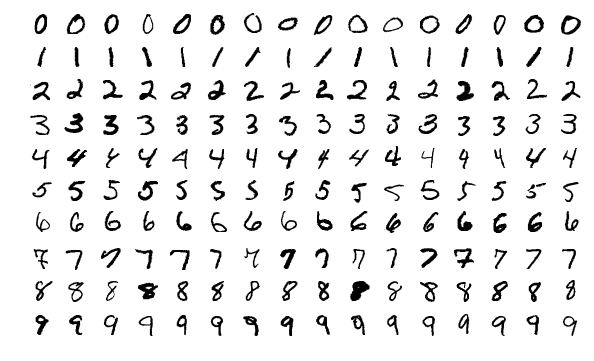
\includegraphics[]{MnistExamples}}
Dataset $D$
}

\end{column}\hfill
\begin{column}{0.7\linewidth}
\centering
\only<1>{
\resizebox{!}{0.5\textheight}{
\neuralnetwork
}
}
\only<2>{
\resizebox{!}{0.8\textheight}{
\neuralnetworkCost
}
}
\only<3>{
\[\frac{1}{n_{D}}\sum_{x \in D} C(x)\]
}
\end{column}
\end{columns}
\end{layout-imageonly}
\end{frame}

% \begin{frame}{Aufbau eines Perzeptrons}
%     \begin{layout-imageonly}
%     \centering
%     \perceptron
%     \end{layout-imageonly}
% \end{frame}
%
% \begin{frame}{Übertragungsfunktion}
% \begin{layout-full}
% \twosplit{
% \begin{block}{Linearkombination}
%     \[net = x_0w_{0} + x_1w_{1} + x_2w_{2} + ... + x_nw_{n}\]
%     \centering oder
%     \[net = \sum_{i=0}^{n} {x_iw_{i}} \]
% \end{block}
% }{
% \centering
% \resizebox{\linewidth}{!}{
% \perceptronFirstHalf
% }
% }
% \end{layout-full}
% \end{frame}
%
%
%
%
% \begin{frame}{Fehlerfunktion}
% \begin{layout-full}
% \begin{block}{Dataset}
% \[
%   X = \Bigl\{(\vec{x_0}, y_0);(\vec{x_1}, y_1);(\vec{x_2}, y_2);(\dots, \dots);(\vec{x_n}, y_n)\Bigl\}
% \]
% \end{block}
% \twosplit{
% \begin{block}{Mean Squared Error}
% \[E=\frac{1}{2}\sum_{i=0}^{n}(y_i-o_i)^2\]
% \end{block}
% }{
% \centering
% \resizebox{\linewidth}{!}{
% \perceptron
% }
% }
% \end{layout-full}
% \end{frame}
%
% \section{Training}
% \begin{frame}{Dataset}
%
% \[
%   X = \Bigl\{(\vec{x_0}, y_0);(\vec{x_1}, y_1);(\vec{x_2}, y_2);(\dots, \dots);(\vec{x_n}, y_n)\Bigl\}
% \]
% \end{frame}
%
% \begin{frame}{Ableitung der Aktivierungsfunktion}
% \begin{layout-full}
% \begin{block}{Ableitung der Sigmoidfunktion}
% \twosplit{
% \[\varphi'(x)=\frac{1}{1+e^{-x}}\cdot(1+\frac{1}{1+e^{-x}})\]
% \centering oder
% \[\varphi'(x)=\varphi(x)\cdot(1+\varphi(x))\]
% }{
% \begin{tikzpicture}
% \begin{axis}[
%   axis lines=center,
%   xtick={-1,1},
%   ytick={0,0.25},
%   xlabel={$x$},
%   ylabel={$y$},
%   xlabel style={below right},
%   ylabel style={above left},
%   xmin=-5.5,
%   xmax=5.5,
%   ymin=-0.25,
%   ymax=0.5]
% \addplot[color=btdl@color@alerted, style = {thick}]{
% 1/(1+exp(-x))*(1-1/(1+exp(-x)))};
% \end{axis}
% \end{tikzpicture}
% }
% \end{block}
% \end{layout-full}
% \end{frame}
%
%
% \section{Topologie}
% \begin{frame}{Einschichtiges feedforward-Netz}
%     \begin{layout-imageonly}
%     \centering
%     \feedforwardNetwork
%     \end{layout-imageonly}
% \end{frame}
%
% \begin{frame}{Mehrschichtiges feedforward-Netz}
%     \begin{layout-imageonly}
%     \centering
%     \deepfeedforwardNetwork
%     \end{layout-imageonly}
% \end{frame}
%
% \begin{frame}{Rekurrentes Netz}
%     \begin{layout-imageonly}
%     \centering
%     \recursiveNetwork
%     \end{layout-imageonly}
% \end{frame}


\end{document}
